\FloatBarrier
\section{Query-Modulated Models Capacity (Simultaneous, Heterogeneous Dimensions)*}

\begin{figure}[!htb]
% \vspace{-0.225in}
\centering
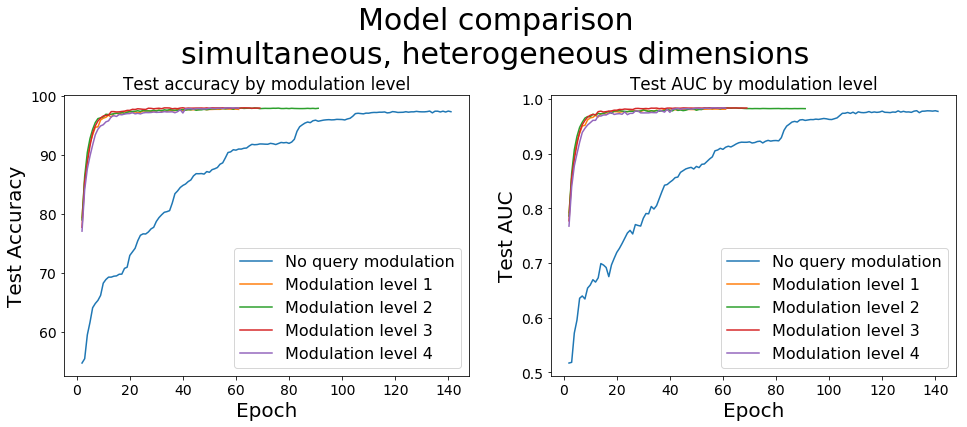
\includegraphics[width=\linewidth]{ch-results/figures/query_mod_simultaneous/baseline_comparison.png}
\caption{ {\bf Baseline to query-modulated model comparison.} Comparing between the baseline model and all four query-modulated models on the simultaneous, heterogeneous dimensions condition. \textbf{Left:} held-out test set accuracy for each model. \textbf{Right:} held-out test set AUC (area under the receiver operating characteristics curve), a more holistic accuracy measure.}
\label{fig:results-query-mod-simultaneous-baseline-comparison}
% \vspace{-0.2in}
\end{figure}

Before we investigated the query-modulated models on the sequential, homogeneous-dimension benchmark condition, we began by evaluating them on the entire dataset, in the simultaneous, heterogeneous dimensions baseline. Just as we hoped to demonstrate that the baseline model can learn the entire task in the more straightforward, simultaneous setting, we wanted to evaluate the query-modulated models to have some understanding of whether or not they contribute to learning in a simple setting. Figure \ref{fig:results-query-mod-simultaneous-baseline-comparison} demonstrates that they do. Query modulation at any of the four convolutional layer groups we examined vastly improves performance, allowing to reach 95\% accuracy and 0.95 AUC within ten epochs, an order of magnitude faster than the baseline, non-query-modulated model. The differences between the different query modulation levels are relatively minuscule. Figures \ref{fig:results-query-mod-simultaneous-query-mod-only} and \ref{fig:results-query-mod-simultaneous-query-mod-zoomed}(in Appendix \ref{sec:additional-figures-query-mod-simultaneous}) focus on the relative performance of these models, demonstrating that query modulation at the third convolution layer appears slightly better for the majority of training, and modulation at the second and fourth levels catch up later in training. We were then curious why these models peak at around 98\% accuracy and 0.984 AUC, and so we split the performance by the individual queries in each dimension.

\begin{figure}[!htb]
% \vspace{-0.225in}
\centering
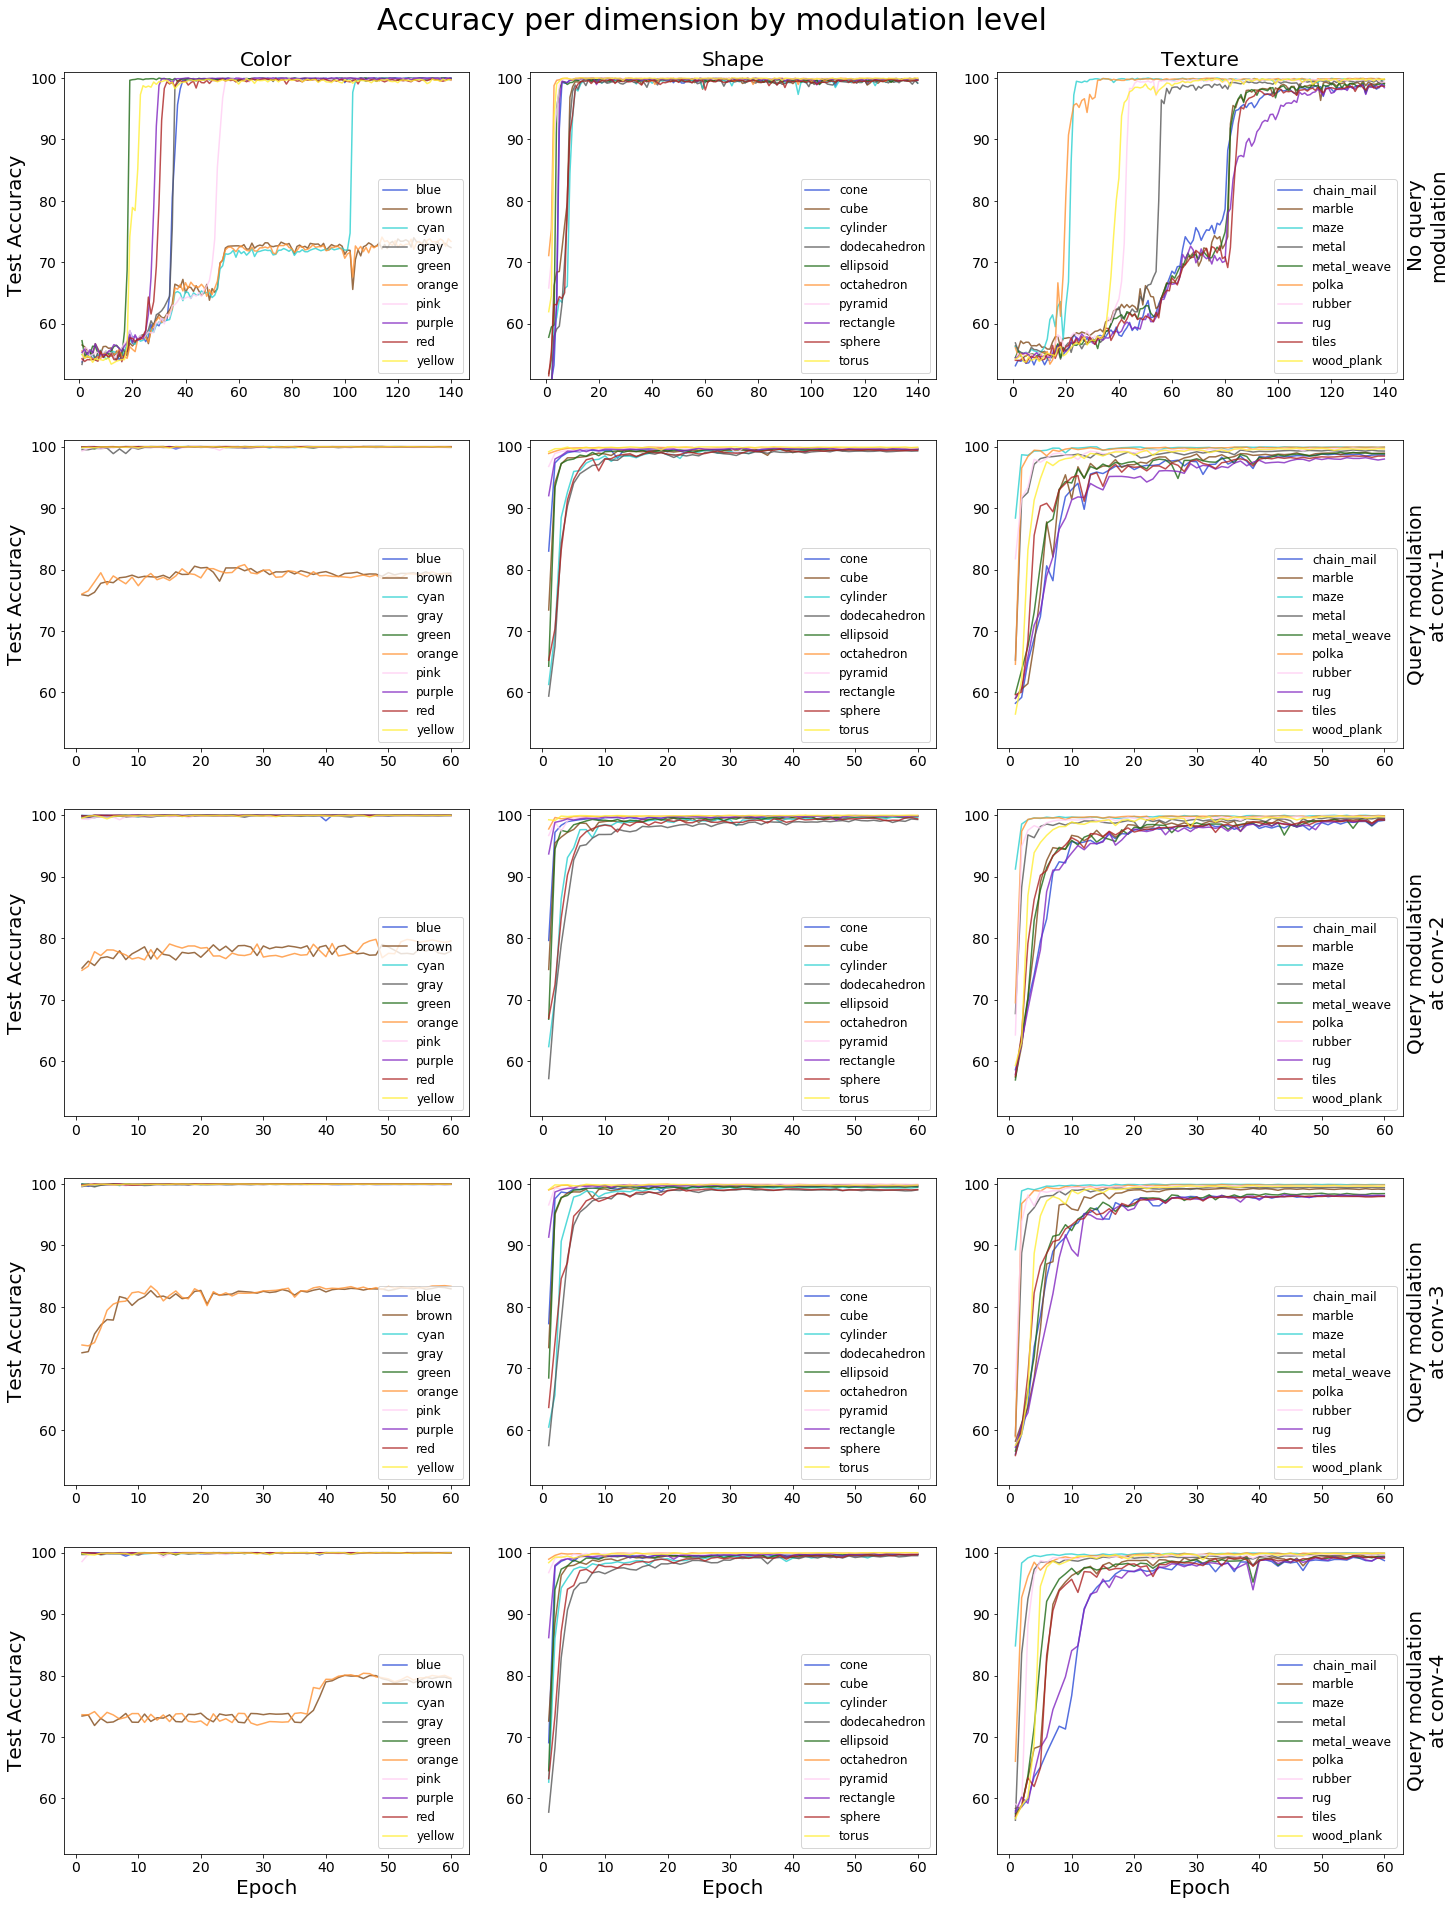
\includegraphics[width=\linewidth]{ch-results/figures/query_mod_simultaneous/query_mod_by_dimension.png}
\caption{ {\bf Test set per-query accuracy split by dimension and model.} For each model (row of plots), we plot the held-out test set accuracy for each dimension (column of plots). Colors used in the plots match the colors used in the dataset. Note that the baseline model, in the top row, received substantially more training epochs than the query-modulating models.}
\label{fig:results-query-mod-simultaneous-query-mod-by-dimension}
% \vspace{-0.2in}
\end{figure}

Figure \ref{fig:results-query-mod-simultaneous-query-mod-by-dimension} depicts the test-set accuracy in each dimensions for each modulation level, and provides some fascinating results. All models struggle with discriminating between brown and orange, peaking at 80\% accuracy when queried on these two colors. The query-modulated models immediately learn to discriminate between the other colors, while the model without modulation acquires them as training proceeds. Shapes challenge the models the least, and all of them reach near-perfect accuracy on shapes early in training. Textures behave more like colors than like shapes, with some variation between the query-modulated models, but all substantially outpace the baseline model, which learns the last texture to 95\% accuracy after around one hundred epochs of training. It is not surprising that query-modulated in the convolution processing aids more with colors and textures than with shapes. Both colors and textures are local properties, which the model could compute from most small patches of an object, and query modulation of the convolutional filters can help tune them to specific features. Conversely, discriminating between shapes requires reasoning about the bounding box of the object, which can only be done by combining information from multiple patches of the convolutional processing, and is most likely best handled by the fully connected module which follows the convolutional processing.
\FloatBarrier